
\documentclass[12pt, a4paper]{article}
\usepackage{hyperref}
\hypersetup{
  colorlinks=true,
  linkcolor=blue,
  urlcolor=cyan,
}
\urlstyle{same}
\usepackage[utf8]{inputenc}
\usepackage{amsmath}
\usepackage{amsfonts}
\usepackage{amssymb}
\usepackage{graphicx}


\newtheorem{theorem}{Teorema.}
\newtheorem{lemma}[theorem]{Lema.}
\newtheorem{corollary}[theorem]{Corolario.}
\newtheorem{definition}[theorem]{Definici\'on:}
\newtheorem{example}[theorem]{Ejemplo:}
\newtheorem{problema}[theorem]{Problema:}
\newtheorem{remark}[theorem]{Observaci\'on:}

\usepackage{graphicx}
\usepackage[spanish]{babel}
%\usetheme{default}

\newcommand{\pp}{\mathbb{P}}
\newcommand{\zz}{\mathbb{Z}}
\newcommand{\rr}{\mathbb{R}}
\newcommand{\qq}{\mathbb{Q}}

\usepackage{tikz, tikz-3dplot}

\definecolor{cof}{RGB}{219,144,71}
\definecolor{pur}{RGB}{186,146,162}
\definecolor{greeo}{RGB}{91,173,69}
\definecolor{greet}{RGB}{52,111,72}

\date{}

\begin{document}
\title{PRÁCTICO 1 LENGUAJES FORMALES: Automatas finitos deterministas (AFDs).}
\author{Mauricio Velasco}
\maketitle{}

\begin{center}
\begin{figure}
\label{Fig}
\caption{Diagramas de estados del problema $(1)$.}
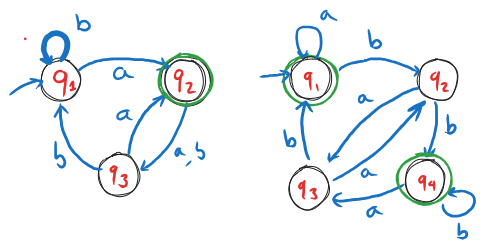
\includegraphics[width=0.8\textwidth]{ADF_1.png}
\end{figure}
\end{center}
\begin{enumerate}
\item Considere los dos diagramas de estados de las máquinas $M_1$ y $M_2$ descritas en la figura~(1) y responda las siguientes preguntas para cada una de ellas:
\begin{enumerate}
\item Cuál es el estado inicial?
\item Cuál es el conjunto de \emph{estados de aceptación}?
\item Qué sucesión de estados tiene cada una de las máquinas al procesar la cadena $\verb!aabb!$?
\item La máquina acepta la cadena $\verb!aabb!$?
\item La máquina acepta la cadena $\epsilon$?
\end{enumerate} 

 
\item La \emph{descripción formal} de un AFD $M$ esta dada por  
\[\left(\{q_1,q_2,q_3,q_4,q_5\},\{u,d\},\delta,q_3,\{q_3\}\right)\] 
donde
\[
\begin{tabular}{c|cc}
\delta & u & d\\
\hline
q_1 & q_1 & q_2\\
q_2 & q_1 & q_3\\
q_3 & q_2 & q_4\\
q_4 & q_3 & q_5\\
q_5 & q_4 & q_5\\
\end{tabular}
\]
Dibuje el diagrama de estados de esta máquina. 

\item Escriba la descripción formal de las dos máquinas del ejercicio $(1)$.
 
\item Demuestre que todo AFD puede convertirse en uno equivalente con un único estado de aceptación (recuerde que dos AFDs son equivalentes si aceptan y rechazan exáctamente las mismas palabras).

\item Suponga que $\Sigma=\{a,b\}$. Construya AFDs para los siguientes lenguajes y demuestre la validez del mismo:
\begin{enumerate}
\item $\{w\in \Sigma^*:\text{$w$ tiene una o dos $b's$}\}$
\item $\{w\in \Sigma^*:\text{$w$ tiene un número par de $a's$}\}$
\end{enumerate}

\item{Usando los AFD que construyó en el ejercicio anterior, construya un AFD para cada uno de los siguientes lenguajes,describa en palabras el lenguaje resultante y justifique la validez de su AFD:
\begin{enumerate}
\item La intersección entre los lenguajes de las partes $(a)$ y $(b)$.
\item La unión entre los lenguajes de las partes $(a)$ y $(b)$.
\item La concatenación de los lenguajes de las partes $(a)$ y $(b)$
\item El complemento del lenguaje de la parte $(b)$
\end{enumerate}



\end{enumerate}
\end{document}



